% !Mode:: "TeX:UTF-8"
%
% 第四章：实现细节
%
% 本节展示的用法：
%   - 多行合并表格（multirow）
%   - 子图排版（subfloat）
%   - 矩阵公式（pmatrix）
%   - 分段函数（cases）
%   - 单图插入
%

\chapter{实现细节}
\echapter{Implementation Details}
\label{chap:implementation}

本章介绍方法的具体实现细节。

\section{数据增强}
\esection{Data Augmentation}
\label{sec:augmentation}

表\ref{tab:aug}列出了使用的数据增强策略。

\begin{table}[h]
\centering
\caption{数据增强策略}
\label{tab:aug}
\begin{tabular}{lcc}
\toprule
增强方法 & 概率 & 参数说明 \\
\midrule
随机旋转 & 0.5 & \([-15^\circ, 15^\circ]\) \\
水平翻转 & 0.5 & — \\
高斯噪声 & 0.3 & \(\sigma = 0.01\) \\
\bottomrule
\end{tabular}
\end{table}

\section{网络架构}
\esection{Network Architecture}
\label{sec:arch}

表\ref{tab:arch}展示了网络结构。

\begin{table}[h]
\centering
\caption{网络架构}
\label{tab:arch}
\begin{tabular}{ccl}
\toprule
\multirow{2}{*}{特征提取}
& 卷积层 \(3\times3\) & 64 通道 \\
& 池化层 & \(2\times2\) \\
\midrule
\multirow{2}{*}{分类头}
& 全连接层 & 256 维 \\
& Softmax 输出 & 10 类 \\
\bottomrule
\end{tabular}
\end{table}

\section{可视化示例}
\esection{Visualization Examples}
\label{sec:vis}

图\ref{fig:single}为单图示例，图\ref{fig:subfigs}为子图排版示例。

\begin{figure}[h]
\centering
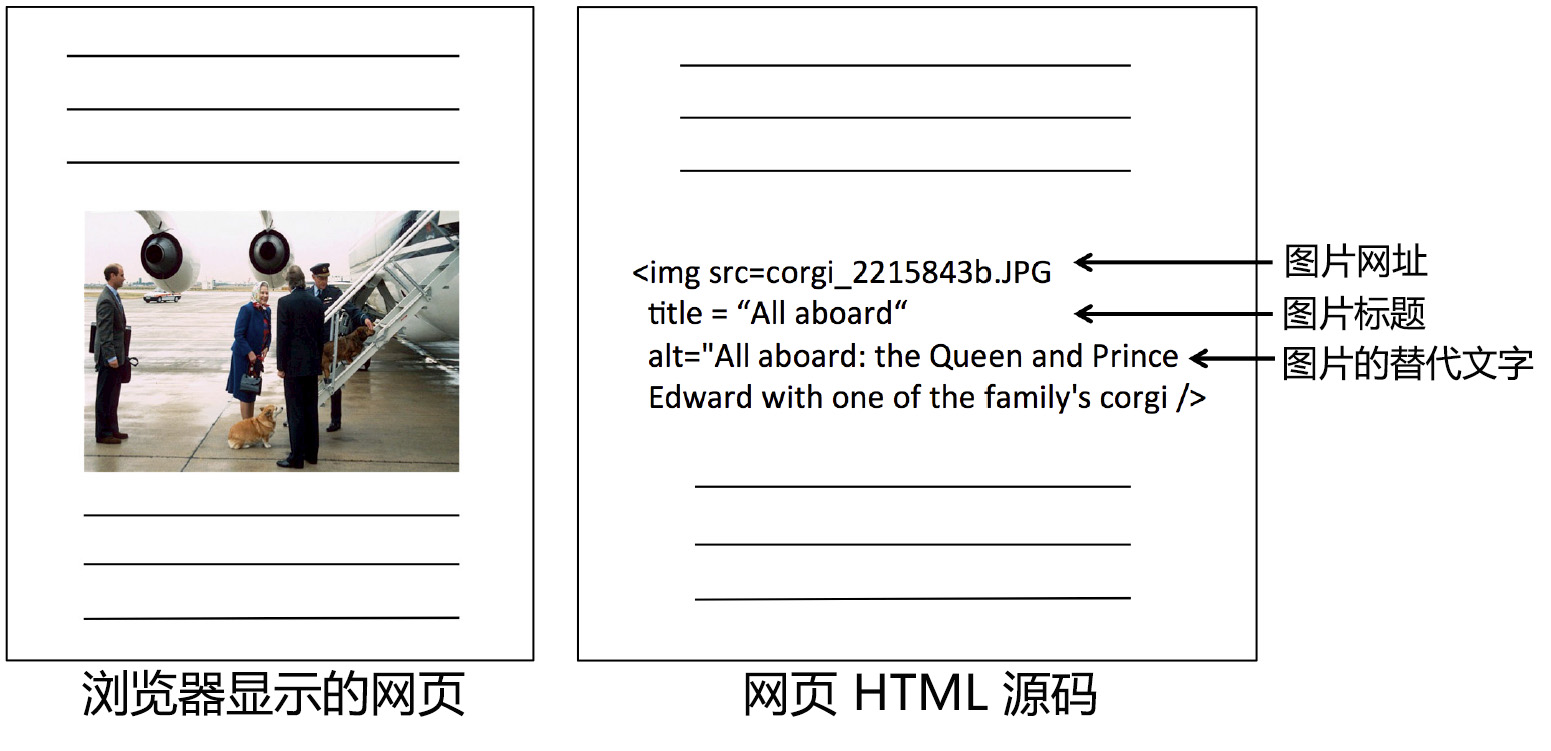
\includegraphics[width=0.5\textwidth]{figures/htmltext}
\caption{单图插入示例}
\label{fig:single}
\end{figure}

\begin{figure}[h]
\centering
\subfloat[子图一]{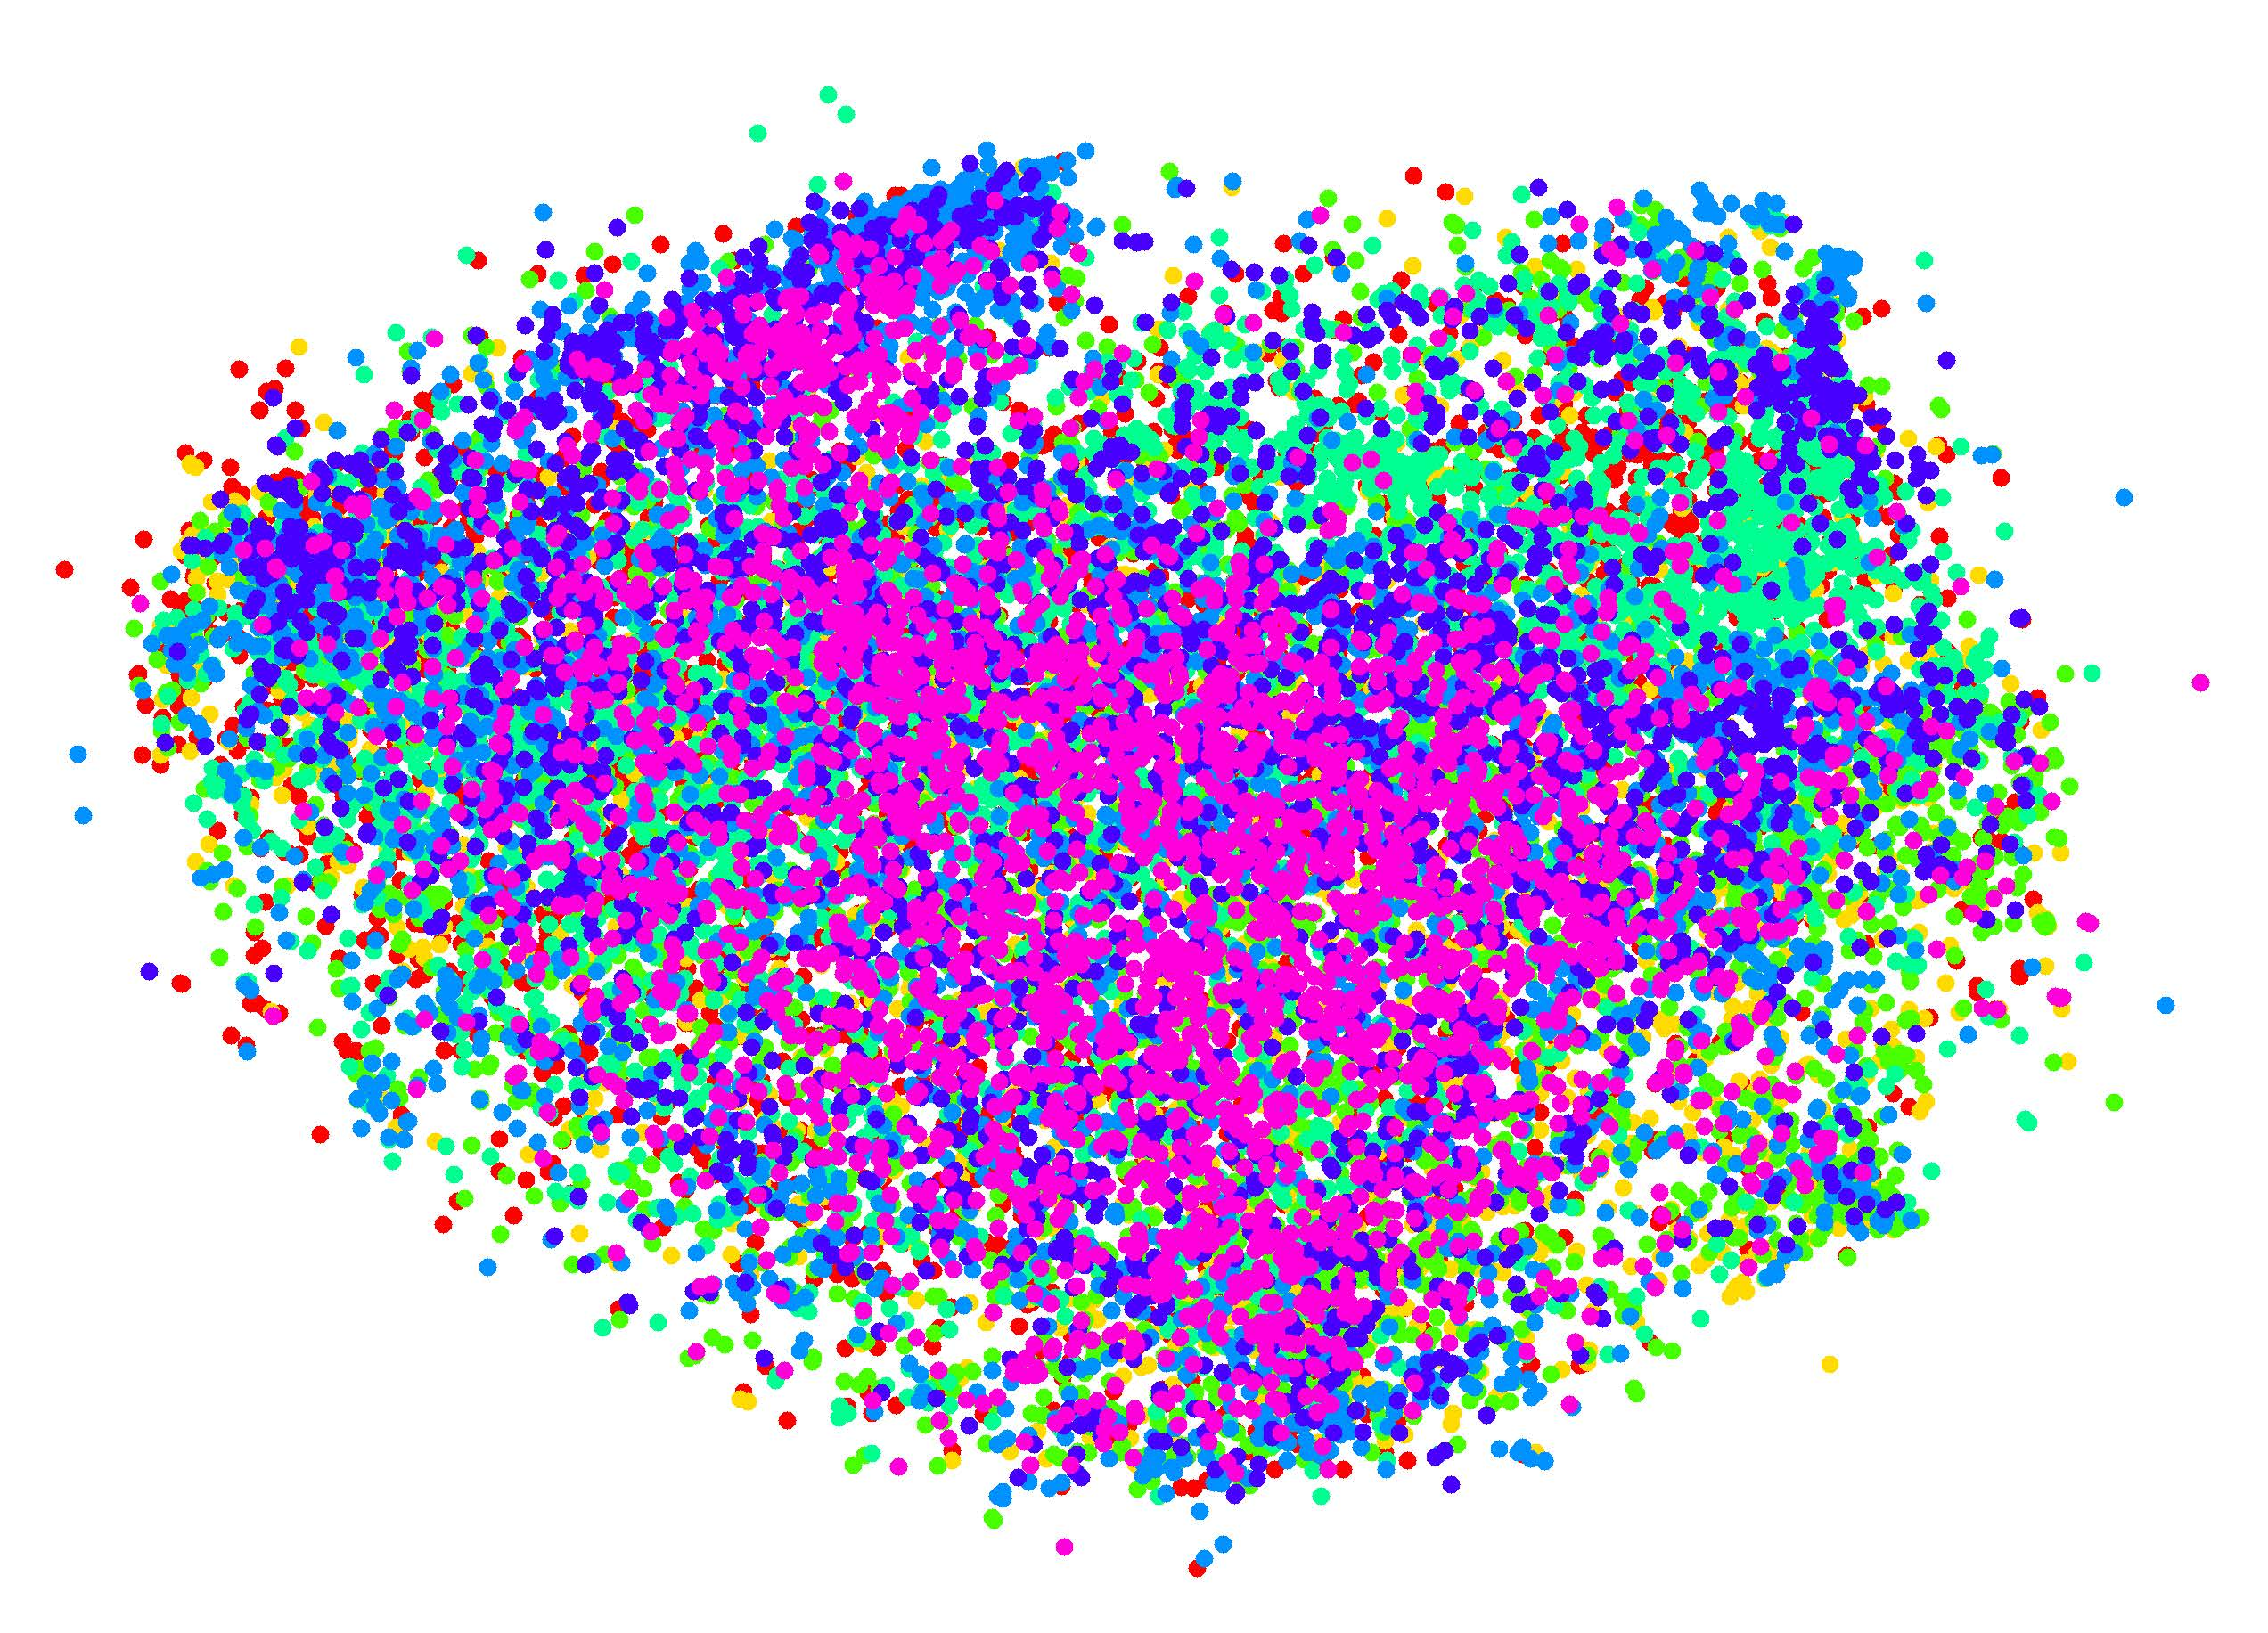
\includegraphics[width=0.28\textwidth]{figures/DECAF1}\label{fig:a}}
\qquad
\subfloat[子图二]{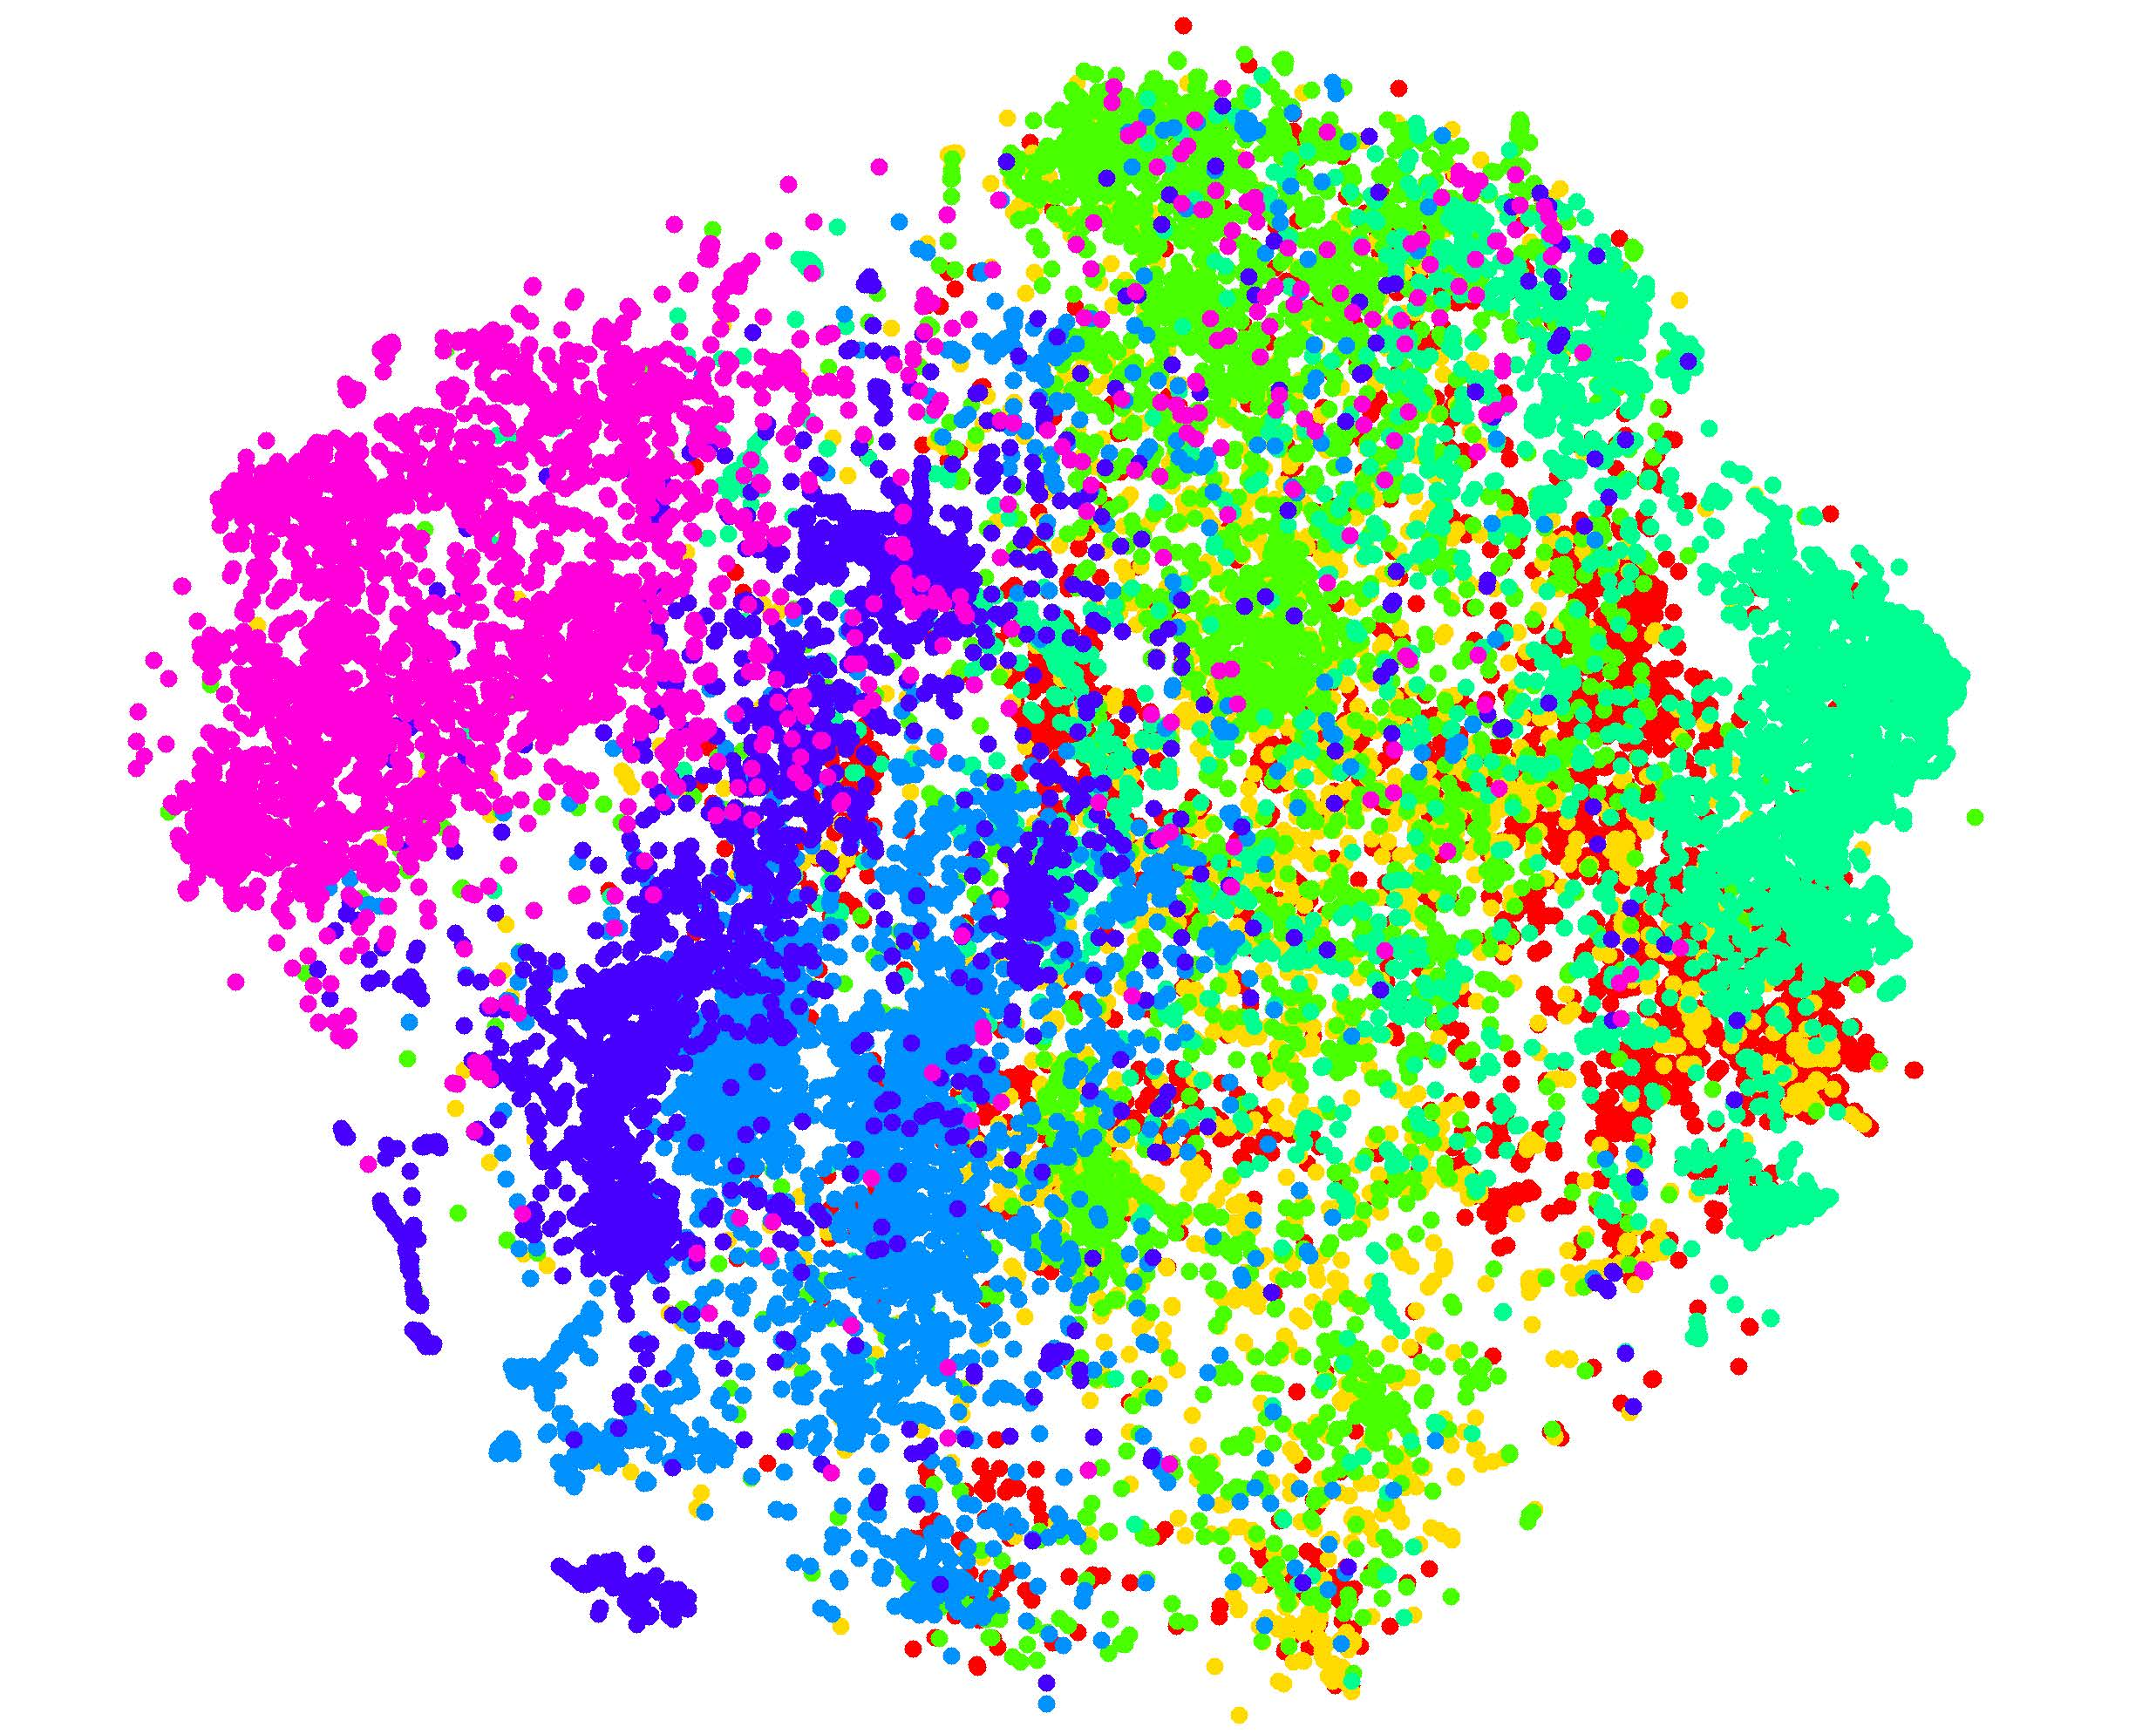
\includegraphics[width=0.28\textwidth]{figures/DECAF6}\label{fig:b}}
\caption{多子图排版示例}
\label{fig:subfigs}
\end{figure}

\section{数学公式}
\esection{Math Formulas}
\label{sec:math}

矩阵与分段函数的写法示例：
\begin{equation}
A = \begin{pmatrix}
a_{11} & a_{12} \\
a_{21} & a_{22}
\end{pmatrix},
\qquad
\frac{\partial u}{\partial t} =
\begin{cases}
\alpha \nabla^2 u, & x \in \Omega,\; t > 0,\\
u_0(x), & t = 0.
\end{cases}
\label{eq:matrix_cases}
\end{equation}
